\documentclass[a4paper,10pt]{article}

\usepackage[utf8]{inputenc}
\usepackage{amsmath,amssymb}
\usepackage[outputdir=../]{minted}
\usepackage{graphicx}
\setlength{\arrayrulewidth}{0.5mm}
\usemintedstyle{borland}
\usepackage{libertine}
\usepackage{xpatch}
\usepackage{booktabs}
\usepackage[backend=biber,style=ieee]{biblatex}
\addbibresource{References.bib}

\renewcommand{\P}{$\mathbb{P}$}
\newcommand{\E}{$\mathbb{E}$}

\makeatletter
% fix for the first kind
\xpatchcmd\inputminted
  {#3}
  {\import@path #3}
  {}{\fail}
% fix for second kind
\xpretocmd\minted@pygmentize
  {\restore@IfFileExists} % direct \let\IfFileExists\im@@IfFileExists works too
  {}{\fail}
\def\restore@IfFileExists{%
  \ifx\IfFileExists\@iffileonpath
    \let\IfFileExists\im@@IfFileExists
  \fi
}
\makeatother
\usepackage{algpseudocode}
\usepackage[linesnumbered,lined,ruled]{algorithm2e}
\usepackage{fancyvrb}
\usepackage{fancyhdr}
\usepackage[skip=0pt]{caption}
\usepackage[a4paper,left=25mm,top=25mm,textwidth=160mm,textheight=249.7mm]{geometry}
\linespread{1.3} 
% \setlength{\baselineskip}{\textheight}
\usepackage[skip=10pt,indent=0pt]{parskip}

\usepackage{array}
\usepackage{calc} % for calculating minipage widths
% Correct order of tables after \paragraph or \subparagraph
\usepackage{etoolbox}
\makeatletter
\def\maxwidth{\ifdim\Gin@nat@width>\linewidth\linewidth\else\Gin@nat@width\fi}
\def\maxheight{\ifdim\Gin@nat@height>\textheight\textheight\else\Gin@nat@height\fi}
\makeatother
% Scale images if necessary so that they will not overflow the page
% margins by default, and it is still possible to overwrite the defaults
% using explicit options in \includegraphics[width, height, ...]{}
\setkeys{Gin}{width=\maxwidth,height=\maxheight,keepaspectratio}
% Set default figure placement to htbp
\makeatletter
\def\fps@figure{htbp}
\makeatother
\setlength{\emergencystretch}{3em} % prevent overfull lines
% Allow footnotes in longtable head/foot
\usepackage{footnotehyper}
\usepackage{footnote}
\usepackage[flushmargin]{footmisc}
\usepackage{enumitem}
\makesavenoteenv{longtable}
\setlength{\emergencystretch}{3em} % prevent overfull lines
\IfFileExists{bookmark.sty}{\usepackage{bookmark}}{\usepackage{hyperref}}
\IfFileExists{xurl.sty}{\usepackage{xurl}}{} % add URL line breaks if available
\urlstyle{same} % disable monospaced font for URLs
\hypersetup{
  hidelinks,
  pdfcreator={LaTeX via pandoc}}

\newcommand{\1}{\mathbf{1}}
\renewcommand{\labelitemi}{$\circ$}
\renewcommand{\labelitemii}{$\circ$}
% ------------------------ Main Doc ------------------------ %


\newcommand{\reminder}[1]{(((\mbox{$\Longleftarrow \star$}{\textbf{#1}} )))}
\newcommand{\RC}[1]{{\color{red}{RC: #1}}}
\newcommand{\OY}[1]{{\color{blue}{OY: #1}}}

% \renewcommand{\savenotes}{}
% \let\savenotes\relax
\begin{document} 
\captionsetup[figure]{hypcap=false}
\pagestyle{fancy}
\fancyhf{}
\fancyhead[L]{2024 Summer Research Overview}

\title{
    \textbf{\huge
        Multi-Period Compliance Mean Field Game \\
        with \\
        Deep FBSDE Solver}}
\medskip
\author{Orange Ao}
\date{October 10, 2024}

\Large\selectfont\maketitle

\vspace{30pt}

\headrule

\vspace{60pt}
% \begin{minipage}[ht]{\textwidth}
% \setlength{\parindent}{10pt}
\large \textit{This is a research report giving big pictures about:}
\textit{
    \begin{enumerate}
        \item the problem we aim to solve
        \item the key methods/algorithms we propose
        \item the main results we get
        \item comparisons between different methods and consequent results
\end{enumerate}}

\vspace{30pt}

\textit{
    Visit my \href{https://github.com/OrangeAoo/PA-MFG-FBSDE}{\textsc{GitHub Repository}}\label{GitHub-Repo} for more math, algorithm details, and code instructions\footnote{Please start an issue at GitHub or reach out to \href{mailto:ya2538@columbia.edu}{me} if you find any problems.}.
    % Please start an issue at GitHub or reach out to \href{mailto:ya2538@columbia.edu}{me} if you find any problems.
    }

% \end{minipage}

\newpage  % ----------------------------------- NEW PAGE ----------------------------------- %

\setlength{\parindent}{0pt}

\section*{\textsc{Abstract}}

\normalsize This work aims to extend the single-period compliance model in \cite{SC} to
multi-period, proposing several tricks to improve the numeric stability of the deep solver for FBSDEs with jumps. First by reproducing the aforementioned research by Campbell Steven, et al.\ (2021), then by considering an additional period to the original model, we make comparisons between long/short-term perspectives when it comes to multi-period production decision-making in renewable electricity certificate markets, as well as between different numeric tricks when it comes to algorithm stability. Meanwhile, some practical takeaways on parameter-tuning are recorded.

\section{Problem Overview}

Conventional numerical solvers are hard-pressed to solve PA-MFG with
market-clearing conditions, which may be faced with the ``curse of
dimensionality'' (Bellman 1957)\footnote{Bellman, R. E.: Dynamic
  Programming. Princeton University Press, USA (1957).}. Thus in their
study \cite{SC}, Professor Campbell and his fellows proposed an actor-critic approach to optimization, where the agents form a Nash equilibria according to the principal's penalty function and the principal evaluates the resulting equilibria. They apply this approach to a stylized PA problem
arising in Renewable Energy Certificate (REC) markets, where agents may
\emph{work} overtime (or \emph{rent} capacity), \emph{trade} RECs, and
\emph{expand} their long-term capacity to navigate the market at maximum
profit. Here we only discuss the agents' problem in the
multi-agent-multi-period scenario.

\subsection{REC Market Basics}

Closely related to carbon cap-and-trade (C\&T) markets, REC markets are
a type of market-based emissions regulation policies, which are
motivating real-world applications of FBSDEs in modeling PA-MFG.

In RES markets, a regulator plays the role of principle, setting a floor
on the amount of energy generated from renewable resources (aka. green
energy) for each firm (based on a percentage of their total production),
and providing certificates for each MWh of green energy generated and
delivered to the grid. These certificates can be further traded by
individual or companies, i.e.~agents, to 1) reduce costs or the
greenhouse gas (GHG) emissions impact of their operations; and 2) earn
profits from the extra inventories instead of wasting. Since the
certificates are traded assets, energy suppliers can trade-off between
producing clean electricity themselves, and purchasing the certificates
on the market. In all, such policies have played an important role in
funding clean energy development, particularly in past years when the
cost of green power production was not as competitive with the cost of
fossil fuel power.

To ensure compliance, each firm must surrender RECs totaling the floor
at the end of a compliance period, with a monetary penalty paid for each
lacking certificate. In practice, these systems regulate multiple
consecutive and disjoint compliance periods, which are linked together
through a mechanism called \emph{banking}, where unused allowances in
current period can be carried on to the next period (or multiple future
periods). Thus, as an extension to the single-period framework \cite{SC}, we
now consider a 2-period model in this report.\footnote{At a finite set
  of joint points, the possible lack of differentiability will not have
  any significant effects.}.

\subsection{REC Market Modeling with
FBSDEs}\label{rec-market-modeling}

Let's consider 2 sub-populations here. Before jumping into the 2-period
case, we first reproduce the single-period case following steps in \cite{SC}. We
denote the period end as \(T\), which can be thought of ``the end of the
world''. Referring to the probabilistic method in \cite{RC} (R. Carmona, F. Delarue,
2012), one can show that, for agent \(i\) in sub-population \(k\), the
optimal solution to its problem in a \emph{single} period is exactly the
solution to the following coupled FBSDEs:


Now consider the 2-agent-2-period MFG with market-clearing conditions.
Let's denote the 2 compliance periods \([0,T_1]\) and \((T_1,T_2]\) as
\(\mathfrak{T_1}\) and \(\mathfrak{T_2}\), respectively. Here we think
of \(T_2\) as ``the end of the world'', after which there are no costs
occurs and all agents forfeit any remaining RECs. Similarly, one can
prove that the optimal operation for agent \(i\) in sub-population
\(k~(\forall~i \in \mathfrak{N}_k,~k\in\lbrace{1,2\rbrace})\) can be
modeled with the following coupled FBSDEs:

\begin{alignat}{2}
    &\begin{cases}
        dX_t^{i} =(h^{k}+g_t^{i}+\Gamma_t^{i}+C_t^{i})dt + \sigma^{k}dW_t^{k} - \min\left(X_{T_1}^i,K\right)\mathbf{1}_{t=T_1},  &X_0^{i} = \zeta^{i} \sim \mathcal{N}(v^k,\eta^k)\\
        dC_t^{i} = a_t^{i}dt ,  &C_0^{k}=0 \\ 
        dV_t^{i} = Z_t^{V,k}dW_t^{i},  &V_{T_1}^{i}=w*\mathbf{1}_{X^i_{T_1}<K} \\
        dU_t^{i} = Z_t^{U,k}dW_t^{i},  &U_{T_1}^{i}=1*Y_{T_1}^i\mathbf{1}_{X^i_{T_1}>K}\\
        dY_t^{i} = Z_t^{Y,k}dW_t^{i},  &Y_{T_2}^{i}=w*\mathbf{1}_{X^i_{T_2}<K}\quad,
    \end{cases} \\
    \textit{where} &\textit{ the optimal controls are given by:}\\
    & S_t = \frac{\sum\limits_{k \in \mathcal{k}} {\frac{\pi^k}{\gamma^k}\mathbb{E}\big[ V_t^i +U_t^i ~|~ i \in \mathfrak{N}^k; \mathcal{F}_t \big]}}{\sum\limits_{k \in \mathcal{K}}{(\pi^k/\gamma^k)}} 
            ~\mathbf{1}_{t\in [0,T_1]} +
            \frac{\sum\limits_{k \in \mathcal{k}} {\frac{\pi^k}{\gamma^k}\mathbb{E}\big[ Y_t^i ~|~ i \in \mathfrak{N}^k; \mathcal{F}_t \big]}}{\sum\limits_{k \in \mathcal{K}}{(\pi^k/\gamma^k)}} 
            ~\mathbf{1}_{t\in (T_1,T_2]} \\
    & g_t^{i} = \frac{V_t^{i}+U_t^{i}}{\zeta^{k}} ~\mathbf{1}_{t\in [0,T_1]}
                + \frac{Y_t^{i}}{\zeta^{k}} ~\mathbf{1}_{t\in (T_1,T_2]} \\
    & \Gamma_t^{i} =\  \frac{V_t^{i}+U_t^{i}-S_t}{\gamma^{k}} ~\mathbf{1}_{t\in [0,T_1]}
                    + \frac{Y_t^{i}-S_t}{\gamma^{k}} ~\mathbf{1}_{t\in (T_1,T_2]} \\
    & a_t^{i} =\frac{(T_1-t)(V_t^{i}+U_t^{i})+(T_2-T_1)Y^i_t}{\beta^{k}} ~\mathbf{1}_{t\in [0,T_1]}
                + \frac{(T_2-t)Y_t^{i}}{\beta^{k}} ~\mathbf{1}_{t\in (T_1,T_2]} \\
\end{alignat}

The parameters for each sub-population are given in the following table:

\begin{table}[ht]
    \centering
    \begin{tabular}{*{9}{c}}
        \toprule
        \, & $\pi^k$ & $h^k$ & $\sigma^k$ & $\zeta^k$ & $\gamma^k$ & $v^k$ & $\eta^k$ & $\beta^k$ \\
        \midrule
        k=1 & 0.25 & 0.2 & 0.1  & 1.75 & 1.25 & 0.6 & 0.1 & 1.0 \\
        k=2 & 0.75 & 0.5 & 0.15 & 1.25 & 1.75 & 0.2 & 0.1 & 1.0 \\
        \toprule
    \end{tabular}
    \caption{Sub-Population Parameter Values}
    \label{tab:Params}
\end{table}

The framework above can be extended to more realistic models with more
than 2 sub-populations and compliance periods, with a penalty approximated
by multi-knot functions.

\section{Algorithm And Numeric
Tricks}

\subsection{Algorithms: Joint-Optimization Vs.
Separate-Optimization}

To solve the said FBSDEs in \ref{rec-market-modeling}, we
implement the \textbf{\emph{shooting method}} with \emph{\textbf{Deep Solvers}}
\cite{JH}, discretizing the SDEs in a fine time grid and parameterizing the
co-adjoint processes and initial values with neural nets. Let
\(\mathfrak{T}=\lbrace{t_0,~...~, t_m \rbrace}\) be a discrete set of
points with \(t_0=0\) and \(T_m=T\), where m is the number of time
steps. Here the step size \(dt=(t_i-t_{i-1})\) is a constant and
\(dt=T/m\). The smaller the value of h, the closer our discretized paths
will be to the continuous-time paths we wish to simulate. Certainly,
this will be at the expense of greater computational effort. While there
are plenty of discretization schemes available, the simplest and most
common scheme is the \emph{Euler scheme}, which is intuitive and easy to
implement. In particular, it satisfies the \emph{practical
decision-making process} - make decisions for the next point of time
conditioned on the current information.

The aforementioned \textbf{\emph{shooting method}} is implemented by the
\textbf{\textit{stepwise approximation}}: starting from the initial conditions and
\emph{"shoot"} for the "correct" terminal conditions - the
``correctness'' of terminal approximations will be evaluated by
computing the aggregated average forward loss/error over the whole
population against corresponding targets (denoted as \(\mathcal{L}\)).
For instance, for the single-period case, the aggregated average forward
MSE after m iterations is computed as: \[
\mathcal{L}(\theta^{(m)})= \sum_{i\in\mathfrak{N}}(Y_{T}^i-w\mathbf{1}_{X_{T}^i<K})^2,
\] and for the 2-period case:

\[
\mathcal{L}(\theta^{(m)})= \sum_{i\in\mathfrak{N}}(V_{T_1}^i-w\mathbf{1}_{X_{T_1}^i<K})^2 + \sum_{i\in\mathfrak{N}}(U_{T_1}^i-Y_{T_1}^i\mathbf{1}_{X_{T_1}^i>K})^2 + \sum_{i\in\mathfrak{N}}(Y_{T_2}^i-w\mathbf{1}_{X_{T_2}^i<K})^2.
\]

The algorithm takes major steps as follows:

\begin{enumerate}
    \item
      start from the neural nets for initial values (i.e.~\(Y_0^i\) etc.);
    \item
      compute the process values at every time step;
    \item
      get approximations to terminal conditions and compute \(\mathcal{L}\);
    \item
      compute gradients of \(\mathcal{L}\) against parameters(weights and
      biases, denoted as \(\theta^{(m)}\)) in the neural nets
      (i.e.~\(Y_0^i\) and \(Z_t^k\) etc.) and take gradient steps to
      determine the next set of parameters.
\end{enumerate}

More specifically, the above steps can be more explicitly displayed by the pseudocode in the \hyperlink{Algorithms}{Appendix} section.

To benchmark the jointly optimized 2-period Model, we first run the 1-period algorithm for each period, i.e. minimize the agents' costs in either period separately. 

% Intuitively, the former algorithm can be interpreted as a long-term perspective, considering the future compliance in the current period and thus planning by investing more in increasing their capacities, even when the first period ends. And the latter one can be seen as a short-sighted approach, caring only for the current quota. These 2 distinctive perspectives can make a huge difference in not only the agents' positions but also the market prices.

% The only difference between the 2 algorithms lies in the \textbf{\textit{stepwise approximation}} when computing forward losses and recording approximated
% paths. Specifically, as is shown in \ref{rec-market-modeling}, there are more additional processes (e.g.~\(V_t^i\)) in the jointly optimized 2-period case. Yet in general, the \textbf{\textit{stepwise approximation}} algorithm can be roughly displayed as the following pseudocode

\subsection{Numeric Tricks}\label{numeric-tricks}

The trickiest problem we are facing is the indicator functions in
\emph{terminal conditions}. Another problem is that the ordinary Deep FBSDE Solver may learn \(V_t^i,U_t^i,Y_t^i \notin [0,1]\) (let's fix \(w=1\) for now), which is meaningless as they represent the \emph{probabilities} of defaulting (i.e.~missing the quota). To solve them, we propose 3 numeric tricks and integrate a combined method into the algorithm.

\paragraph{Sigmoid Approximation} A natural way to increase continuity and differentiability is by (see Figure \ref{fig:sig-approx} in the \hyperlink{Algorithms}{Appendix} section):
\begin{equation}
    \1_{0.9>x} \approx \sigma(0.9-x), ~\textit{where the sigmoid function}~\sigma(u)=\frac{1}{1+e^{-u/\delta}}.
\end{equation}

In particular, the parameter \(\delta\) controls the steepness of
\(\sigma(\cdot)\) and usually is a small positive number - the smaller
\(\delta\) is, the more closely it approximates the step of the indicator function. 

\paragraph{Numeric Clamp} Instead of using \texttt{tensor.clamp} to brutally clamp values within \([0,1]\), we introduce a more numerically stable way, especially for values close to the 2 interval ends (same applies to \(V_t^i, U_t^i\)).

\begin{equation}\label{dY_tilde}
    dY_t^i=Y_t^i(1-Y_t^i)Z_tdB_t.
\end{equation}

Nonetheless, there are limitations to the above approaches. For the \textit{sigmoid approximation}, when \(\delta\) is too small, there is a great potential for numerical overflow - the exponents could be tremendous especially when \(X_t\) is far greater than 0.9, such that \texttt{torch.exp(u)} is \texttt{inf} when
$u \ge 7.1$. This will raise errors/warnings\footnote{Examples of
  \href{https://discuss.pytorch.org/t/second-order-derivative-with-nan-value-runtimeerror-function-sigmoidbackwardbackward0-returned-nan-values-in-its-0th-output/173260}{RuntimeError}
  and
  \href{https://discuss.pytorch.org/t/output-overflow-and-unstablity-when-use-model-eval/3668}{RuntimeWarning}
  on PyTorch Forums.} in PyTorch. And for \textit{numeric clamp} to work, we must ensure the \textbf{initial values} strictly fall in \((0,1)\). Thus we propose the third approach:

\paragraph{Logit Clamp Transformation} To map the range $[0,1] \to \mathbb{R}$ while avoids working with large exponents, we let:
$\tilde{Y} := w*\text{logit} (Y/w)$. Then apply \(\textit{It}\hat{o} \textit{'s formula}\) (with
superscript \([\cdot]^i\) omitted):

\begin{equation}
    d \tilde{Y}_t = (w/2-Y_t)Z_t^2dt + wZ_tdB_t~.
\end{equation} 

Correspondingly, we use \href{https://pytorch.org/docs/stable/generated/torch.nn.BCEWithLogitsLoss.html}{\textit{BCEWithLogitsLoss}} as the loss function, which combines a Sigmoid layer and the \textit{BCELoss} in one single class. This version is more numerically stable than using a plain \textit{Sigmoid} followed by a  \textit{BCELoss} as, by combining the operations into one layer, it takes advantage of the log-sum-exp trick for numerical stability.

Worth mentioning, we experimented with multiple combinations of tricks
and loss functions, paired with different optimizers and schedulers.
Eventually, we chose
\href{https://pytorch.org/docs/stable/generated/torch.optim.Adamax.html}{\texttt{Adamax}}
and
\href{https://pytorch.org/docs/stable/generated/torch.optim.lr_scheduler.StepLR.html}{\texttt{StepLR}}
due to their relatively better and more stable performance for all cases
in general. Specifically, the 4 valid combinations of tricks and
loss functions are shown as follows.

\begin{table}[ht]
    \centering
    \begin{tabular}{*{4}{c}}
        \toprule
        \, & \textbf{target type} & \textbf{trick} & \textbf{loss type} \\
        \midrule
        1 & indicator & logit & BCEWithLogitsLoss \\
        2 & indicator & clamp & BCELoss \\
        3 & indicator & clamp & MSELoss \\
        4 & sigmoid   & clamp & MSELoss \\
        \toprule
    \end{tabular}
    \caption{Valid Combos}
    \label{tab:valid-combos}
\end{table}



\newpage

\section{Results}\label{results}

To facilitate the evaluation of algorithm performances, \texttt{plot\_results} - a
user-friendly class - is constructed.\footnote{See more instruction details in GitHub \href{https://github.com/OrangeAoo/PA-MFG-FBSDE/blob/3cffc5e8dbe09fbc880f6c2c70d76e0b6a1b8c3c/2Period/Joint_Optim_2Prdx1/README.md}{README} for the Joint-Optimization or Separate-Optimization.}, which also visualizes agents' behaviors (or interactions) and their market impacts. Specifically, it produces results from the following aspects:

\vspace{-0.5\topsep}

\begin{itemize}
  \setlength{\parskip}{0pt}
  % \setlength{\itemsep}{-8pt}
  \item\textbf{Agents' behaviors and market impacts}
    \begin{itemize}
      % \setlength{\itemsep}{-10pt}
      \item Learnt optimal control processes
      \item Decomposed inventory accumulation processes
      \item Inventory levels during 2 compliance periods
      \item Terminal inventories ready-to-submit
      \item Market-clearing prices
    \end{itemize}
  \item\textbf{Algorithm convergency and learning loss}
      \begin{itemize}
        \item Average forward losses against a number of epochs trained
        \item Learnt terminal conditions vs. targets
      \end{itemize}
\end{itemize}

And here are some example diagrams.

\subsection{Jointly Optimized 2-Agent-2-Period Sample Results}

Here we use the sample results by model\footnote{The code and full results can be found in the \href{https://github.com/OrangeAoo/PA-MFG-FBSDE/blob/FBSDE/2Period/Joint_Optim_2Prdx1/Adamax_clamp_sig_MSE.ipynb}{GitHub Repository}.} with terminal target function: $0.25\,\sigma{\left(0.9-X_T^i\right)}$, where $\delta=0.03$ and $T=T_1,\,T_2$. The loss function is \textit{MSELoss} and the trick used in the \textbf{\textit{stepwise approximation}} is \textit{clamp}, correspondingly. (See Table \ref{tab:valid-combos}.)

The learned controls are shown as the first row of Figure \ref{fig:decomp-gen-jnt} and the accumulative generations by different means as the second row, correspondingly. The green color denotes the sub-population 1 while red the sub-population 2. (The same applies to all the later plots.) 
The plots in Figure \ref{fig:terminal-values-jnt} display a rather good convergence of learned terminal values to their \textit{sigmoid targets}. 

% \newpage  % ----------------------------------- NEW PAGE ----------------------------------- %
% \begin{minipage}[ht]{\textwidth}
\begin{center}
\begin{minipage}[ht]{0.8\textwidth} 
    % \centering
    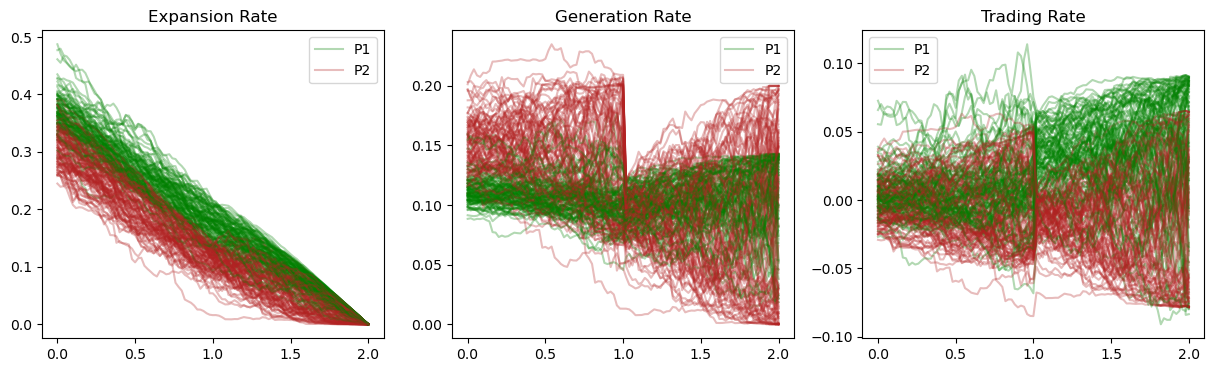
\includegraphics{FinalReports/Illustration_diagrams/Joint-2A2P-Sigmoid-ResExamples/Rates.png}\\
    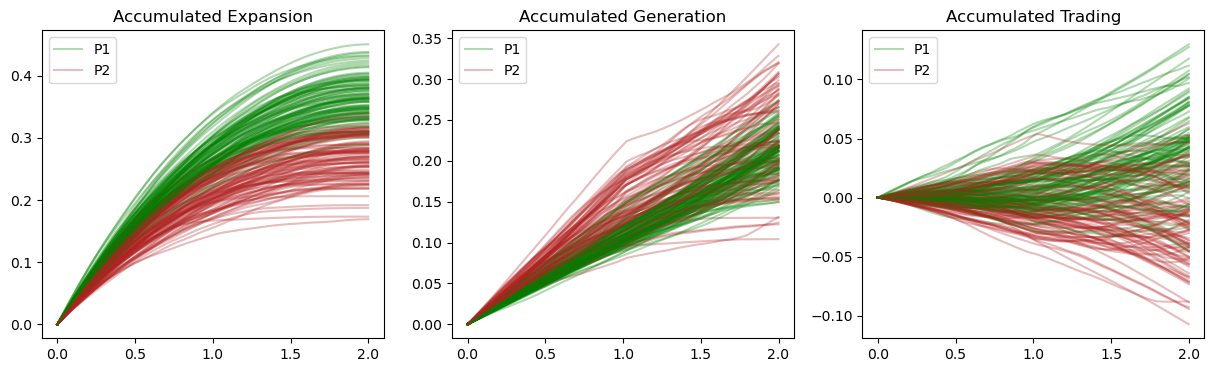
\includegraphics{FinalReports/Illustration_diagrams/Joint-2A2P-Sigmoid-ResExamples/AccumRates.png}\\
    \vspace*{-10pt}
    \captionof{figure}{Decomposed Generation of Joint-Optimization}
    \label{fig:decomp-gen-jnt}
\end{minipage}
\end{center}  

\vfill

\begin{center}
\begin{minipage}[ht]{0.85\textwidth}
    % \centering
    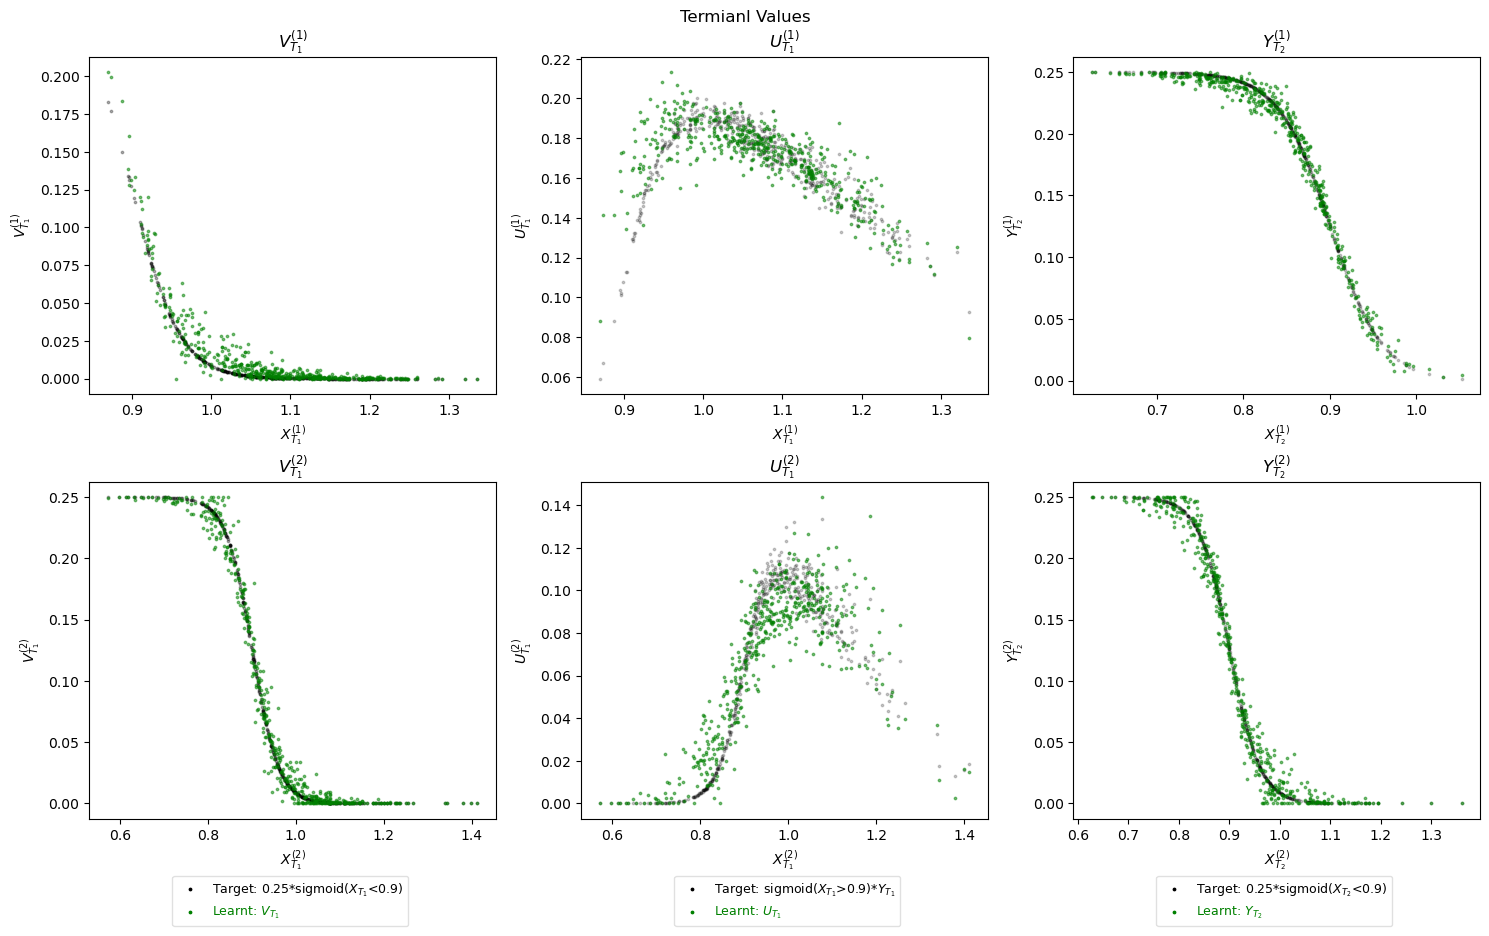
\includegraphics{FinalReports/Illustration_diagrams/Joint-2A2P-Sigmoid-ResExamples/sigmoid_target.png}\\
    \vspace*{-10pt}
    \captionof{figure}{Terminal Values of $V, U, Y$}
    \label{fig:terminal-values-jnt}
\end{minipage}    
\end{center}

\subsection{Separately Optimized 2-Agent-2-Period Sample Results}

For the sake of comparability, here we use the same numeric trick, target, and loss function, except for minor changes when fine-tuning the specific model parameters\footnote{The code and full results can be found in the \href{https://github.com/OrangeAoo/PA-MFG-FBSDE/blob/FBSDE/2Period/Separate_Optim_1Prdx2/Adamax_clamp_sig_MSE.ipynb}{GitHub Repository}.}.


% \begin{minipage}{\textwidth}
\begin{center}
  \begin{minipage}[ht]{0.9\textwidth}
    \centering
    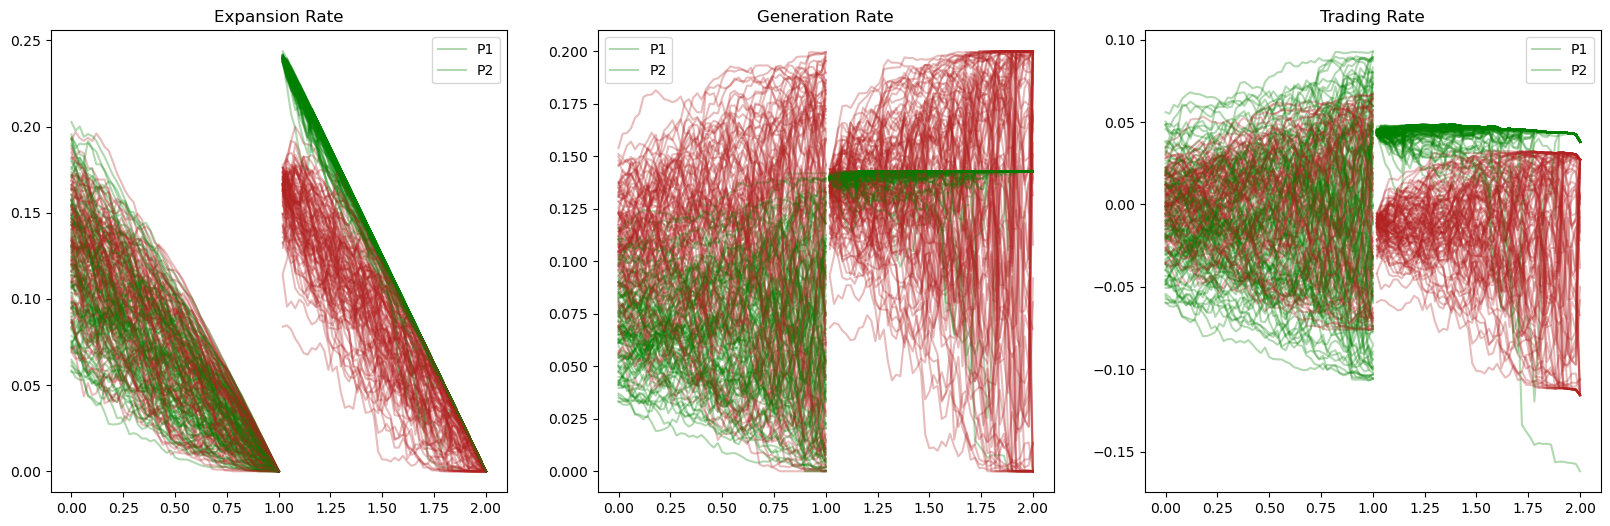
\includegraphics[]{FinalReports/Illustration_diagrams/Seprt-2A2P-Sigmoid-ResExamples/Rates.png}\\
    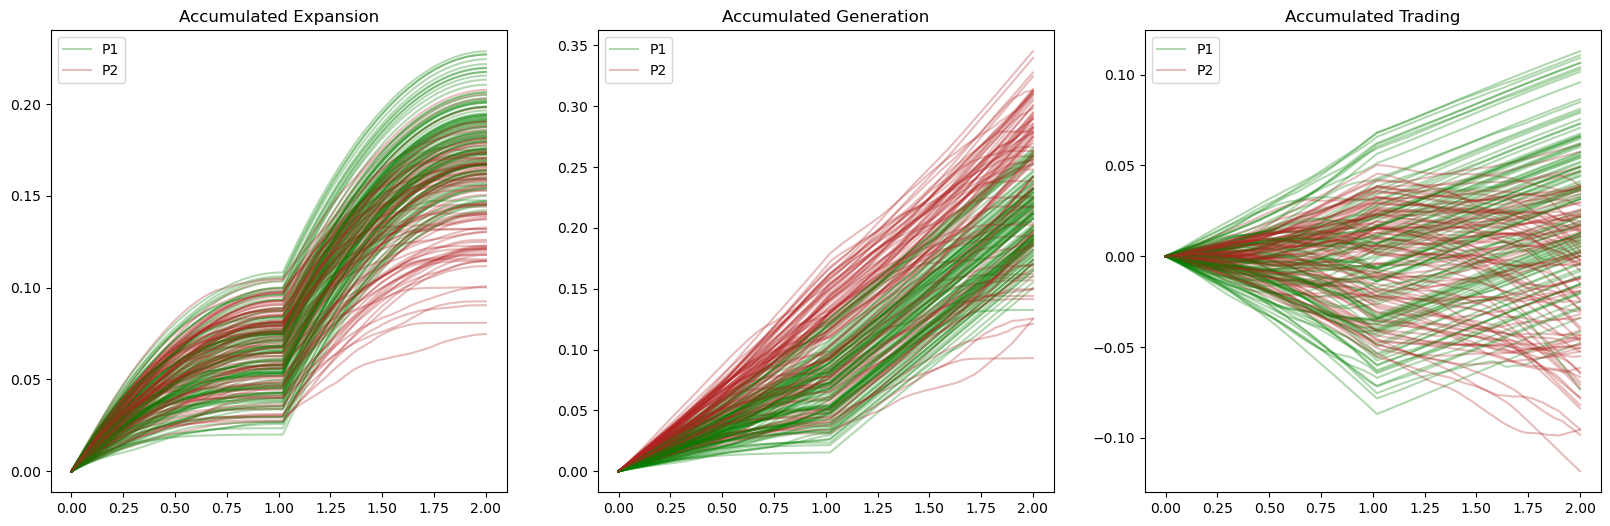
\includegraphics[]{FinalReports/Illustration_diagrams/Seprt-2A2P-Sigmoid-ResExamples/AccumRates.png}\\
    \captionof{figure}{Decomposed Generation of Separate-Optimization}
    \label{fig:decomp-gen-sep}
  \end{minipage}
  
  \begin{minipage}[ht]{0.85\textwidth}
    \centering
    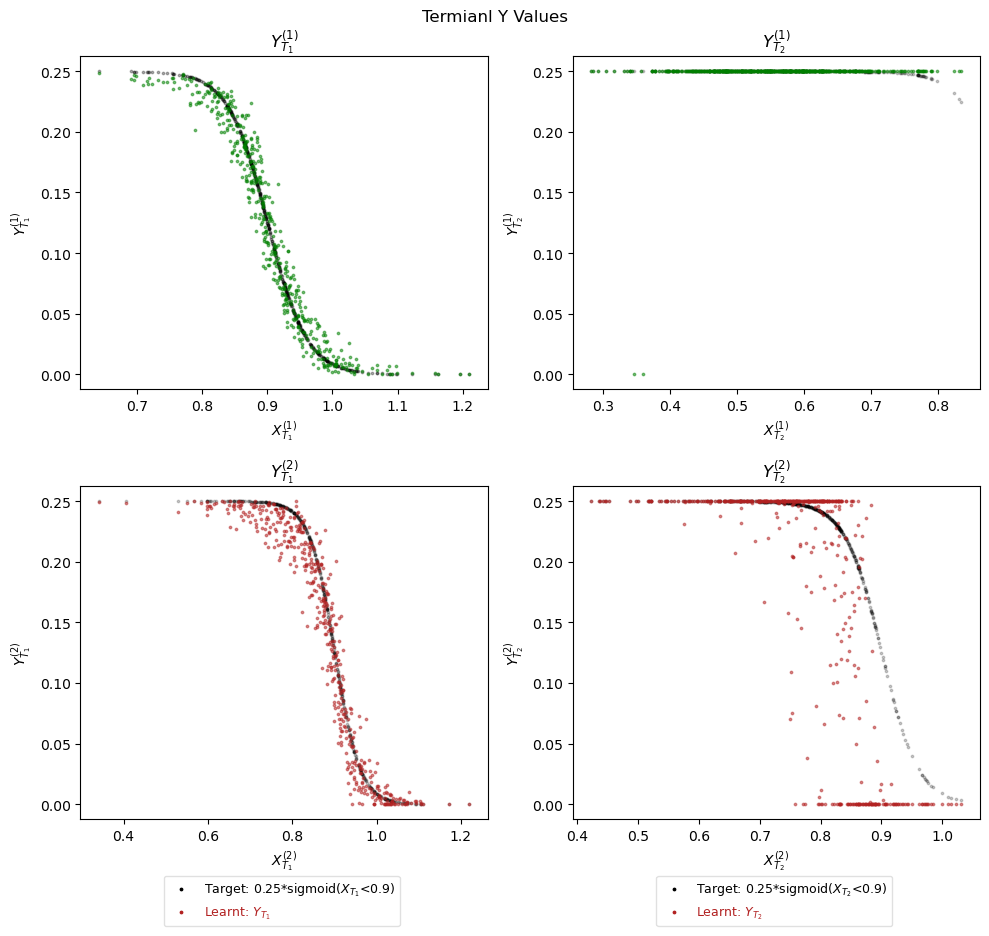
\includegraphics[]{FinalReports/Illustration_diagrams/Seprt-2A2P-Sigmoid-ResExamples/sigmoid_target.png}\\
    \captionof{figure}{Terminal Values of $Y$}
    \label{fig:terminal-values-sep}
  \end{minipage}
\end{center}
% \end{minipage}


\subsection{Comparisons And Analyses}

\paragraph{Joint Vs Separate Optimization}

Upon comparing the shown results from 2 different perspectives, one can
get enlightening implications.

In contrast to the short-sighted agents, those who plan ahead in \textbf{\(\mathfrak{T}_1\)} tend to invest more in expansion even at the end of the first period, generating slightly more than the quota required.

% , whereas when only dedicated to meeting the current target, all
% agents reduce the expansion rate to zero since there's no point
% investing in delayed payoffs. Similarly, the short-sighted agents will
% trade more actively and might work more overtime at the first-period end
% in seek of immediate paybacks. Consequently, most of these agents
% unaware of the upcoming second compliance period will end up ``just''
% meet the quota of 0.9 at \(T_1\), since any extra inventory would be
% regarded ``useless'' - yet find themselves having to start over from
% almost scratch to meet the second quota. This can be seen from
% the first columns of inventory histograms and the inventory level plots.

Therefore in \textbf{\(\mathfrak{T}_2\)}, they are saved from starting from scratch. And since most of them have already accumulated a relatively high baseline rate, there's less need to work overtime or purchase inventories than in the first period (shown by the decreased slopes of the accumulated generation plots). However, the agents in the benchmark model have to either 1) try very hard to make up for expansion (exemplified by the green ``pop1''), or 2) rely heavily on over-hours and trading (exemplified by the red ``pop2'').

Consequently, their market impact will be reflected by the trading prices: the greater the demand, the higher the prices. 

\begin{center}
\begin{figure}
    \centering
    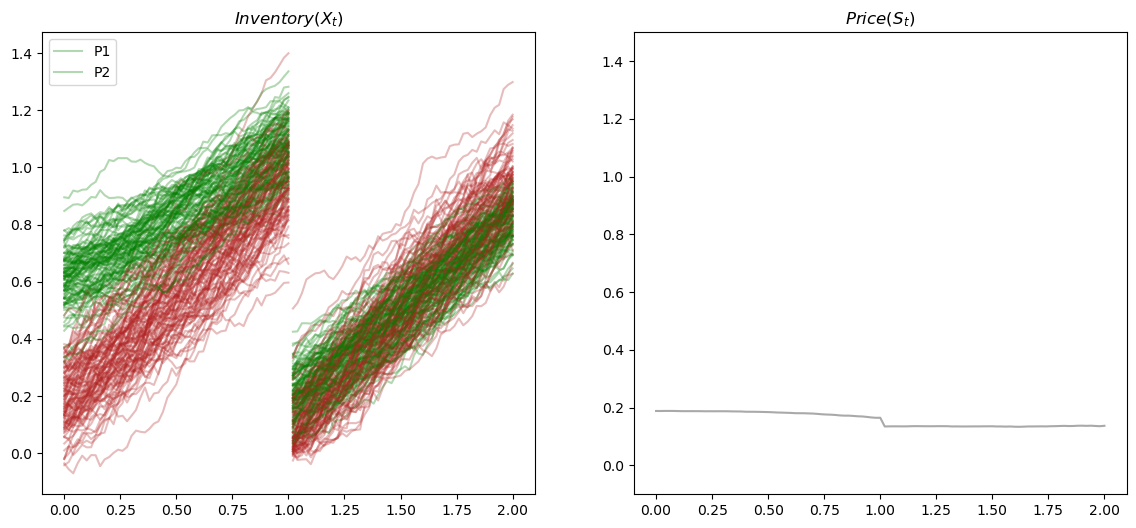
\includegraphics[]{2Period/Joint_Optim_2Prdx1/Illustration_diagrams/InvAndPrice.png}
    \caption{Market Price Comparison}
    \label{fig:price}
\end{figure}
\end{center}

\paragraph{Sub-Population 1 Vs 2}

Then let's take a closer look at either case, analyzing the differences
made by distinctive preferences and initial conditions across
sub-populations. Starting at generally lower initial level (\(v^1>v^2\))
yet blessed with greater baseline rate (\(h^1<h^2\)), ``pop2'' wouldn't
worry as much as the green guys ``pop1'' in terms of expansion, and find
working overtime or trading more rewarding. Even further, the red guys
would be more interested in overtime than in trading since it's
``cheaper'' per unit inventory, which is the opposite for the green guys
(i.e.~\(\zeta^1>\gamma^1, \zeta^2<\gamma^2\)).

However, regardless of agents' perspectives (long/short-term), the
the explicit initial advantage in inventory level and the implicit
the disadvantage in baseline capacity makes the green guys ``lazier'',
i.e. less motivated to work extra hours. Consequently, in the second
compliance period, they are more likely to find themselves hard-pressed
to meet the quota and have to purchase from the red guys, which is
indicated by the trends and signs (positive for buying and vice versa)
of accumulated trading amount.

\paragraph{Model Performances}

Both algorithms produce descending loss plots and learned terminal
conditions that almost overlap with their targets (black dots) given
\(X_{T_1}^i, X_{T_2}^i\), which suggests converging and stable
of model performance as desired. Worth mentioning, since \textit{sigmoid targets} with \textit{MSELoss} have the greatest differentiability, combined with small \(w\) (e.g. 0.25) narrowing down the step from 0 to \(w\), models set up as such would produce rather good-looking results. Certainly, there might be other parameter and model settings leading to greater
convergence and stability, which are open for experimenting.

\newpage  % ----------------------------------- NEW PAGE ----------------------------------- %
\section{Conclusions And Takeaways}

\paragraph{Conclusions} 

\paragraph{Enlightening Takeaways} From the results and analysis above, one can take away some instructive
implications and apply not only to the REC markets but also to one's daily life.
\textit{\begin{itemize}
  \setlength{\itemsep}{-5pt}
  \item
    Always plan ahead and consider for the future.
  \item
    Always do slightly more than required and maintain a reasonable level
    of backups.
  \item
    Don't be blinded by the apparent advantages/achievements, instead care
    for the growth rate and capacity - that's what you can carry to the
    future for sure.
  \item
      When the majority gets lazy or short-sighted, the market gets worse - where any individual will be affected more or less.
\end{itemize}
}

\newpage
\section*{Appendix}
\subsection*{FBSDEs For The Single-Period-2-Agent Model}

\begin{alignat}{2}
    &\begin{cases}
        dX_t^{i} = (h^{k} + g_t^{i} + \Gamma_t^{i} + C_t^{i})dt + \sigma^{k}dW_t^{k},  &X_0^{i} \sim \mathcal{N}(v^k,\eta^k) \notag \\
        dC_t^{i} = a_t^{i}dt, &C_0^{i}=0 \notag \\
        dY_t^{i} = Z_t^{k}dW_t^{k}, &Y_{T}^{i} = w\mathbf{1}_{X_{T}^i<K}, \notag \\
    \end{cases}\\
    \textit{where:}&\\
        &Y_t^i = \mathbb{E} \left[w\mathbf{1}_{X_{T}^i< K}|\mathcal{F}_t \right] = w\mathbb{P}\left(X_{T}^i< K ~|~ \mathcal {F}_t\right) \notag \\
        &S_t = \frac{\sum\limits_{k \in \mathcal{K}} {\left(\frac{\pi^k}{\gamma^k}\mathbb{E}\left[ Y_t^i ~|~ i \in \mathfrak{N}^k; \mathcal{F}_t \right]\right)} }{\sum\limits_{k \in \mathcal{K}}{\left(\frac{\pi^k}{\gamma^k}\right)}} \notag \\
        &g_t^k = \frac{Y_t^k}{\zeta^k} \notag \\
        &\Gamma_t^{k} = \frac{Y_t^{k}-S_t}{\gamma^{k}} 
\end{alignat}


\subsection*{Key Notations}

The key notations/parameters in the FBSDEs are interpreted as follows:
\begin{itemize}
\item
  \(k \in \mathcal{K}\): a sub-population of agents, within which all
  individuals are assumed to have identical preferences and similar
  initial conditions/capacities, yet across which are distinct. The
  sub-population is annotated by superscript \([\cdot]^{k}\). Here we
  only discuss \(k=1,2\).
\item
  \(i \in \mathfrak{N}\): an individual agent belonging to the
  sub-population \(\mathfrak{N}^k\), annotated by superscript
  \([\cdot]^{i}\).
\item
  \(X_t := (X_t)_{t\in\mathfrak{T_1} \cup \mathfrak{T_2}}\): the current
  inventories in stock. For some key time points:

  \begin{itemize}
  \item
    at \(t=0\), there may be some stochastics in the initial
    inventories, which are assumed to be normally distributed.
    \(X_0^{i} \sim \mathcal{N}(v^k, \eta^k) ,~ \forall k \in \mathcal{K},~\forall i \in \mathfrak{N}^k\).
  \item
    at \(t=T_1\), the terminal RECs pre-submission are \(X_{T_1}\)
    carried over from the first period. Shortly after forfeiting
    \(\min\Big(K,X^i_{T_1}\Big)\), the remaining inventories in stock
    are \(ReLU\Big(X^i_{T_1}-K\Big)\), which are treated as new initial
    values for the second period.
  \item
    at \(t=T_2\), the terminal RECs pre-submission are \(X^i_{T_2}\).
  \end{itemize}
\item
  \(I_t := (I_t)_{t\in\mathfrak{T_1} \cup \mathfrak{T_2}}\): the
  integrated inventory generation. We introduce this process for
  continuous differentiability at \(T_1\). And \(X_t\) has the same
  initial conditions as \(I_t\). We have:

\begin{align}
    X_t=
    \begin{cases}
        I_t\, ,                  \quad& t \in [0,T_1]\\
        I_t- \min(I_{T_1},K)\, , \quad& t \in (T_1,T_2]\\
    \end{cases} 
    \quad\text{or}\quad
    X_t=
    \begin{cases}
        I_t\, ,                       \quad& t \in [0,T_1]\\
        I_t-I_{T_1}+(I_{T_1}-K)_+\, , \quad& t \in (T_1,T_2].\\
    \end{cases} 
\end{align}

    
\item
  \(K\): the quota that agents must meet at the end of each compliance
  period. Fixed to \(K=0.9\)\footnote{The choice of knot point is
    associated with \(h^{k}\) and total time span \(T_1\), \(T_2\). A
    good target (or quota) should be \textbf{``attainable''} - neither
    too easy nor too hard to achieve. Specifically, even if agents do
    nothing at all, they will have an initial amount plus a baseline
    generation of inventories - for instance, \(0.2*1 + 0.6=0.8\) for
    agents in sub-population 1 at the first-period end. Similarly, for
    sub-population 2, all agents will also have a \emph{``guaranteed''}
    level of 0.8 for delivery. Thus a target reasonably higher than
    that, i.e.~0.9, would be regarded \textbf{``attainable''}.}.
\item
  \(P(\cdot)\): the generic penalty function approximated by
  \emph{\textbf{single-knot penalty functions}} \footnote{See
    \href{../FinalReports/Report-StepwiseDetail.md}{\emph{Report-StepwiseDetail}}
    for more math details.} :
  \[P(x)=w(0.9-x)_+ \Rightarrow\partial_{x}P(x) = - w\mathbf{1}_{x<K}.\]
  Further, by tuning the weight \(w\), we can see the relation between
  the penalty level (controlled by \(w\)) and the agents' behaviour, as
  well as its market impact.
\item
  \(h\): the baseline generation rate at which agents generate inventories with zero
  marginal cost.
\item
  \(C_t := (C_t)_{t\in\mathfrak{T_1} \cup \mathfrak{T_2}}\): incremental
  REC capacity of agents, i.e. increase of baseline generation rate
  over time, accumulated by investing in expansion plans - for instance,
  by installing more solar panels. \footnote{The incremental capacity
    over baseline can be carried forward to future periods.}
\item
  \(a_t := (a_t)_{t\in\mathfrak{T_1} \cup \mathfrak{T_2}}\): the control
  of expansion rate, representing long-term REC capacity added per unit
  time. Note that it could be made even more realistic by incorporating
  a \emph{delay} between the decision to expand (\(a_t\)) and the
  increase to the baseline rate \(h\).
\item
  \(g_t := (g_t)_{t\in\mathfrak{T_1} \cup \mathfrak{T_2}}\): the control
  of overtime-generation rate, i.e. extra capacity achieved by
  working extra hours and/or renting short-term REC generation capacity
  at an assumed quadratic cost - specifically, over-hour bonus and/or
  rental fees.
\item
  \(\Gamma_t := (\Gamma_t)_{t\in\mathfrak{T_1} \cup \mathfrak{T_2}}\):
  the control of trading rate, with negative\footnote{While trading rate
    may be positive or negative, expansion and overtime-generation rates
    must be positive.} values being the amount sold whereas positive
  purchased per unit of time.
\item
  \(S_t := (S_t)_{t\in\mathfrak{T_1} \cup \mathfrak{T_2}}\): the
  equilibrium REC price obtained endogenously through market-clearing
  condition:
  \[\lim\limits_{N \to \inf}{\frac{1}{N} \sum\limits_{i\in\mathfrak{N}}{\Gamma^i_t}}=0\]
\item
  \(\zeta,~\gamma,~\beta\): scalar cost parameters which are identical
  for agents within the same sub-population.
\item
  \(\pi\): the proportion of each sub-population:
  \[\pi^k=\frac{|\mathfrak{N}^k|}{\sum\limits_{j \in \mathcal{K}}{|\mathfrak{N}^j|}}.\]
\end{itemize}

\newpage
\hypertarget{Algorithms}{\subsection*{Algorithms}}

The stepwise function to approximate the discretized coupled FBSDEs and the main algorithm - forward training loop - is structured correspondingly as:

\begin{algorithm}[ht]
\SetKwData{batch}{batch}\SetKwData{MaxBatch}{MaxBatch}\SetKwData{OptimSteps}{OptimSteps}
\SetKwData{loss}{loss}\SetKwData{ToTLoss}{ToTLoss}
\SetKwFunction{CalLoss}{CalTerminalLoss}
\SetKwData{dB}{dB}
\SetKwData{v0model}{v0\_model}\SetKwData{zvmodels}{zv\_models}
\SetKwData{u0model}{u0\_model}\SetKwData{zumodels}{zu\_models}
\SetKwData{y0model}{y0\_model}\SetKwData{zymodels}{zy\_models}
\SetKwFunction{getforwardloss}{get\_forward\_loss}
\SetKwFunction{AppendToForwardLosses}{AppendToForwardLosses}
\SetKwProg{Fn}{Function}{\string:}{}
\SetKwInOut{Input}{Input}\SetKwInOut{Output}{Output}
\Input{Initial conditions and untrained models}
\Output{Aggregated forward loss \ToTLoss}
\BlankLine
\Fn{\getforwardloss{initial conditions and models}}{
    Initialization\;
    \For{j $\gets$ 1 \KwTo $T_2$}{
        Update $\mathbb{P}$ (default) for each sub-population:\\
        $V_j \gets V_{j-1}$ + \zvmodels[j-1]*\dB$_j$,
        $\,\,U_j \gets U_{j-1}$ + \zumodels[j-1]*\dB$_j$,
        $\,\,Y_j \gets Y_{j-1}$ + \zymodels[j-1]*\dB$_j$\;
        Compute overtime-generation, trading, and expansion rates: $g$, $\Gamma$, and $a$\;
        Update C and X\;
        \If{j=$T_1$}{
            Freeze X, V, and U at $T_1$\;
            Submit inventories: X $\gets$ ReLU(X - K)\;
        }
    }
    Aggregate the losses: \ToTLoss $\gets$ \CalLoss(V,U,Y)\;
    \KwRet{\ToTLoss}
}
\caption{Shooting Method - Stepwise Approximation} 
\label{alg:stepwise-approx}
\end{algorithm}

\begin{algorithm}[ht]
\LinesNumbered
\SetAlgoLined
\SetKwData{batch}{batch}\SetKwData{MaxBatch}{MaxBatch}\SetKwData{OptimSteps}{OptimSteps}
\SetKwData{loss}{loss}\SetKwData{Loss}{Loss}\SetKwData{SumLoss}{SumLoss}\SetKwData{FL}{forward\_losses}
\SetKwFunction{getforwardloss}{get\_forward\_loss}\SetKwFunction{AppendToForwardLosses}{AppendToForwardLosses}
\SetKwProg{Fn}{Function}{:}{}
\SetKwInOut{Input}{Input}\SetKwInOut{Output}{Output}
\Input{Sample $X_0$, $C_0$, and BM Increments $dB$ for each sub-population}
\Output{Trajectories of $X_t$, $g_t, \Gamma_t, a_t, C_t$, and terminal conditions $V_{T_1}, U_{T_1}, Y_{T_2}$}
\BlankLine
\Begin{
    Initialization\;
    \For{batch $\leftarrow 0$ \KwTo \MaxBatch}{
        \SumLoss $\gets 0$\;
        \For{iter $\leftarrow 0$ \KwTo \OptimSteps}{
            Compute forward loss: \loss $\gets$ \getforwardloss{initial conditions}\;
            Backpropagate: \loss.backward()\;
            Update parameters: optimizer.zero\_grad(), optimizer.step()\;
            Adjust learning rate: schedular.step()\;
            \SumLoss $\gets$ \SumLoss + \loss\;
        }
        \AppendToForwardLosses{\SumLoss/\OptimSteps}\;
        \If{not train on the single batch}{
            Generate a new batch with updated initial processes\;
        }
    }
    \BlankLine
    Visualize the results: Forward Losses, $X_t$, $g_t, \Gamma_t, a_t, C_t$, and terminal convergence.
}
\caption{Training Loop for Forward Loss Approximation}
\label{alg:TrainLoop}
\end{algorithm}

\subsection*{Sigmoid Approximation}

\begin{figure}[ht]
    \centering
    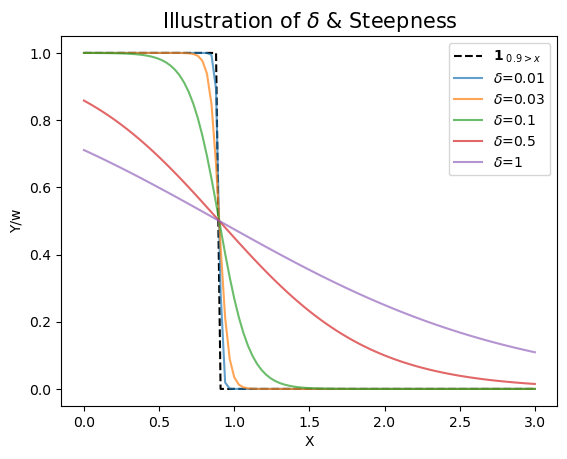
\includegraphics[width=0.5\textwidth]{FinalReports/Illustration_diagrams/SigmoidApprox.png}
    \caption{Sigmoid Approximation}
    \label{fig:sig-approx}
\end{figure}

\newpage  % ----------------------------------- NEW PAGE ----------------------------------- %
\printbibliography 

\end{document}

